\Chapter{Megjelenítési módok}

Az eredmények megjelenítésére már a korábbiakban is sor került. Ez a fejezet külön egységként vizsgálja, hogy a Python, főként a \texttt{matplotlib} segítségével milyen segítséget ad az adatok vizualizálásához.

\Section{Egyszerű grafikonok rajzolása}
    
Ahogy a szoftvereszközök bemutatásánál már volt róla szó, az adatok
vizualizálása nagyon fontos, hisz egy-egy ábráról gyakran könnyebb adatokat
leolvasni, mint nagy táblázatokból vagy egyéb adastruktúrákból.
Python-ban a \texttt{matplotlib} függvénykönyvtárt használhatjuk ezeknek az ábráknak a
létrehozásához.

    Először vegyünk egy egyszerű példát, amelyben bizonyos \(x\) értékekhez
rendeljünk hozzá \(f(x) = y\) értékeket.
\begin{python}
import matplotlib.pyplot as plt
import numpy as np

x = np.zeros(20)
y = np.zeros(20)

for i in range(-9, 10):
    x[i] = i
    y[i] = pow(x[i], 2)
    
plot = plt.plot(x, y, "o")
\end{python}
    A \texttt{matplotlib} \texttt{plot} hívásával tudjuk kirajzoltatni az
ábráinkat, melynek az első paramátere a értelmezési tartomány, a második
az értékkészlet, és további paramáterként meg lehet neki adni a jelölés
formáját, illetve feliratokat a label paraméter segítségével.

Az értékeket megadhatjuk függvény segítségével is, például
\begin{python}
import matplotlib.pyplot as plt
import numpy as np

x = np.zeros(20)
y = np.zeros(20)

for i in range(-9, 10):
    x[i] = i
    
plot=plt.plot(x ,abs(x),"-", label='x abszolut erteke', markersize=10)
plot = plt.legend()

plt.show(plot)
\end{python}
Ennek az eredménye \aref{fig:abs-plot}. ábrán látható.

\begin{figure}[h!]
\centering
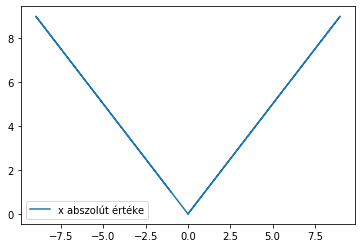
\includegraphics[scale=1.0]{img/abs-plot.png}
\caption{Függvény kirajzolása a \texttt{matplotlib} segítségével.}
\label{fig:abs-plot}
\end{figure}

    Megváltoztathatjuk a színét is az adott ábránknak, illete több függvényt
is ábrázolhatunk egyszerre, például
\begin{python}
import matplotlib.pyplot as plt
import numpy as np
from matplotlib.pyplot import figure

x = np.zeros(100)
d = -4
i = 0
while i < 100:
    x[i] = d;
    d = d + 0.1
    i = i + 1
    
plt.figure(figsize=(18.5, 10.5), dpi=150)
plot = plt.plot(x,np.cos(x), "-r", label='cos x')
plot = plt.plot(x,np.sin(x), "-g", label='sin x')
plot = plt.legend()
plt.show(plot)
\end{python}
Az eredmény \aref{fig:sin-plot}. ábrán szerepel.

\begin{figure}[h!]
\centering
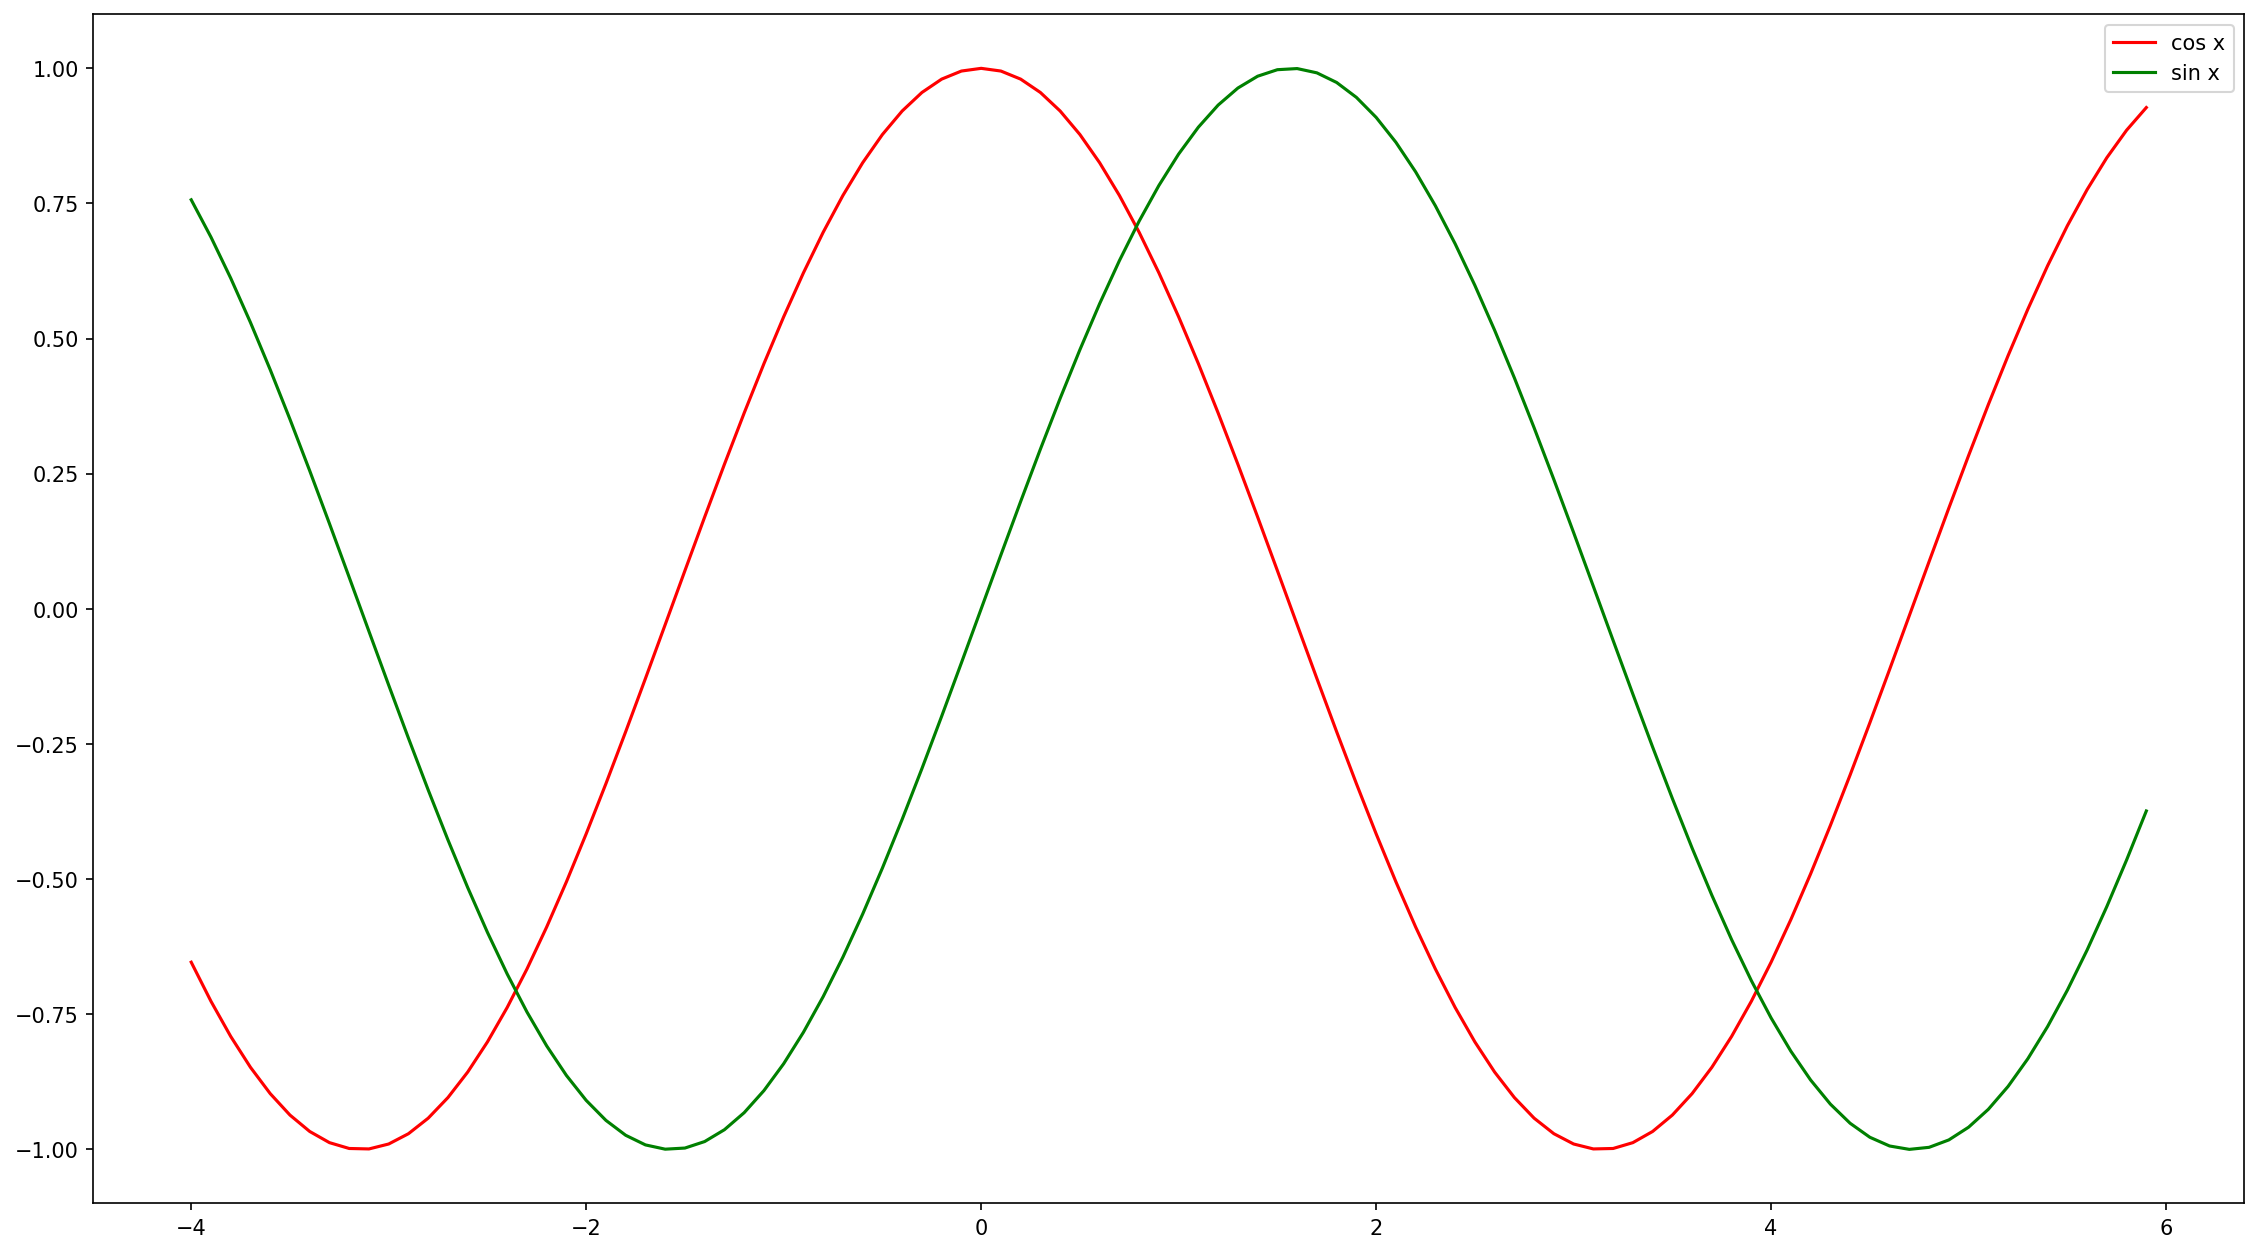
\includegraphics[width=\textwidth]{img/sin-plot.png}
\caption{Több függvény egyidejű kirajzolása.}
\label{fig:sin-plot}
\end{figure}

    Az előző kódrészben importáltam a \texttt{figure}-t a \texttt{matplotlib}
csomagból. Ennek segítségével képesek vagyunk beállítani az ábra
alapvető tulajdonságait, úgy mint például a méretet, de beállíthatjuk a háttér és
szélek színeit vagy a felbontást.

A tengelyeket is elnevezhetjük könnyedén a matplotlib \texttt{ylabel} és
\texttt{xlabel} metódusaival és adhatunk címet is az ábránknak a
\texttt{title} metódussal.

Létrehozhatunk hisztogrammokat is, továbbá adatainkat egy ploton belül töbféleképpen is megjeleníthetjük:
\begin{python}
test = ['1', '2', '3', '4', '5', '6']
points = [68, 70, 75, 76, 80, 78]

plt.figure(figsize=(18.5, 10.5), dpi=150)

plt.subplot(131)
plt.bar(test, points, color='b')
plt.subplot(132)
plt.scatter(test, points, marker='*', color='r')
plt.subplot(133)
plt.plot(test, points, color='black')

plt.show()
\end{python}
Az eredménye \aref{fig:multi-plot}. ábrán látható.

\begin{figure}[h!]
\centering
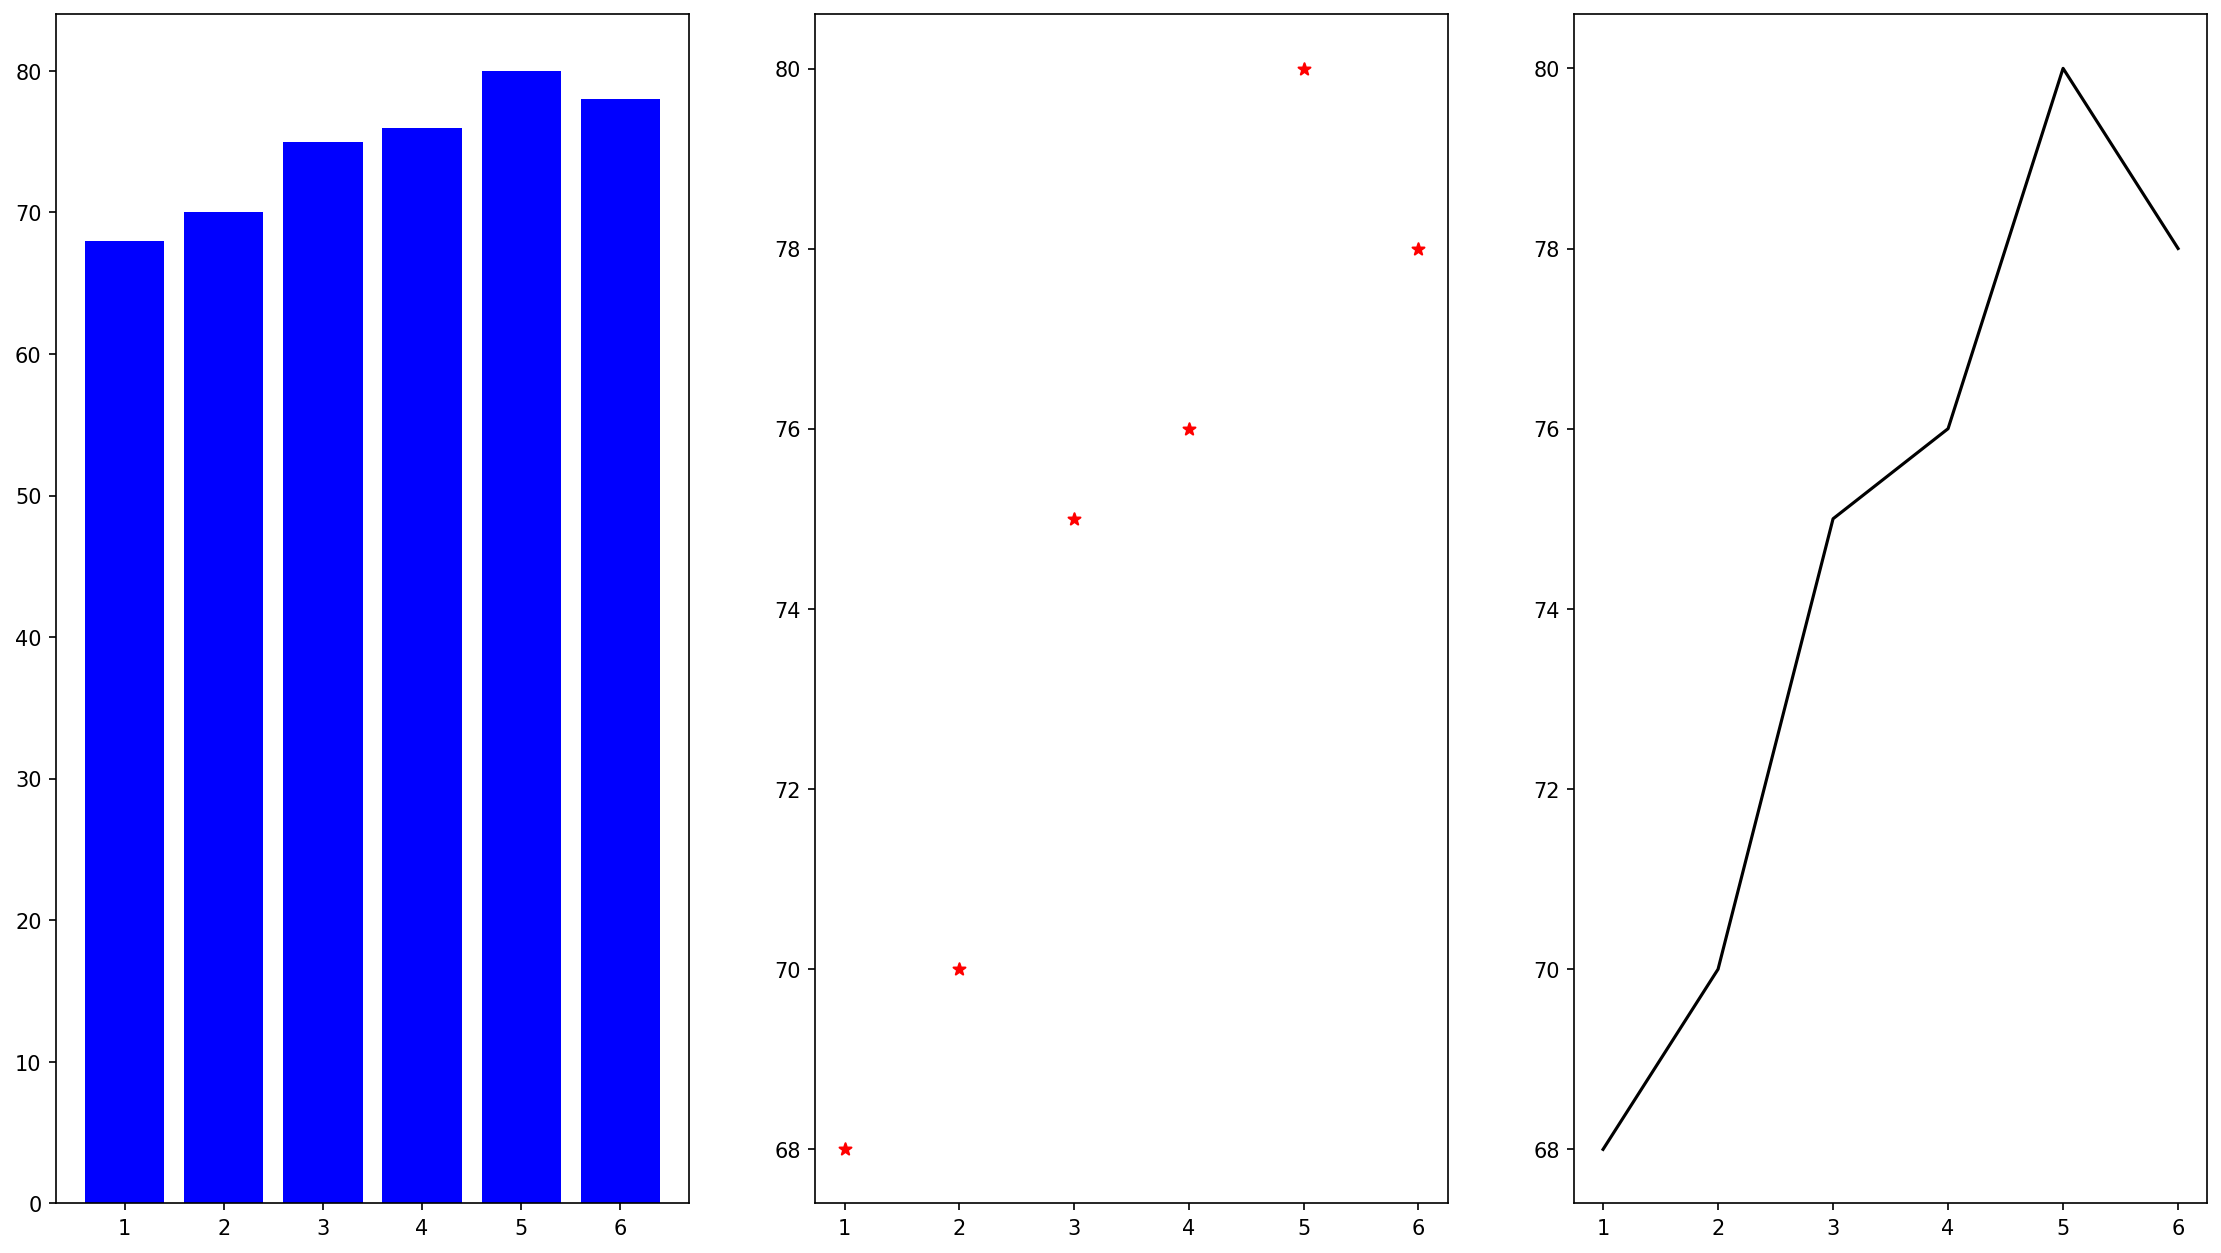
\includegraphics[width=\textwidth]{img/multi-plot.png}
\caption{Több grafikon megjelenítése egymás mellett.}
\label{fig:multi-plot}
\end{figure}
    
    Ilyen esetben a a jelőlő pontokat a \texttt{marker}, míg a színt a \texttt{color} paraméterrel tudjuk megváltoztatni.
    
\Section{Térbeli pontok szemléltetése}

    A Matplotlib megengedi számunkra az is, hogy térbeli pontokat képezzünk le ábráinkon. Ezek lehetnek felületek  térben elszórt pontjai vagy egyéb függvények is. Ehhez szügségünk van a \textbf{mplot3d} csomagra
ami az \textbf{mpl\_toolkits} része.
Először nézzünk meg egy térbeli ívet!
\begin{python}
import matplotlib.pyplot as plt
from mpl_toolkits.mplot3d import axes3d

fig = plt.figure(figsize=(18.5, 10.5), dpi=150)
ax = fig.add_subplot(111, projection='3d')

theta = np.linspace(-4 * np.pi, 4 * np.pi, 100)
z = np.linspace(-2, 2, 100)
r = z**3 + 1
x = r * np.sin(theta)
y = r * np.cos(theta)
ax.plot(x, y, z)
plt.show()
\end{python}
A kirajzolás eredménye \aref{fig:curve-1}. ábrán látható.

\begin{figure}[h!]
\centering
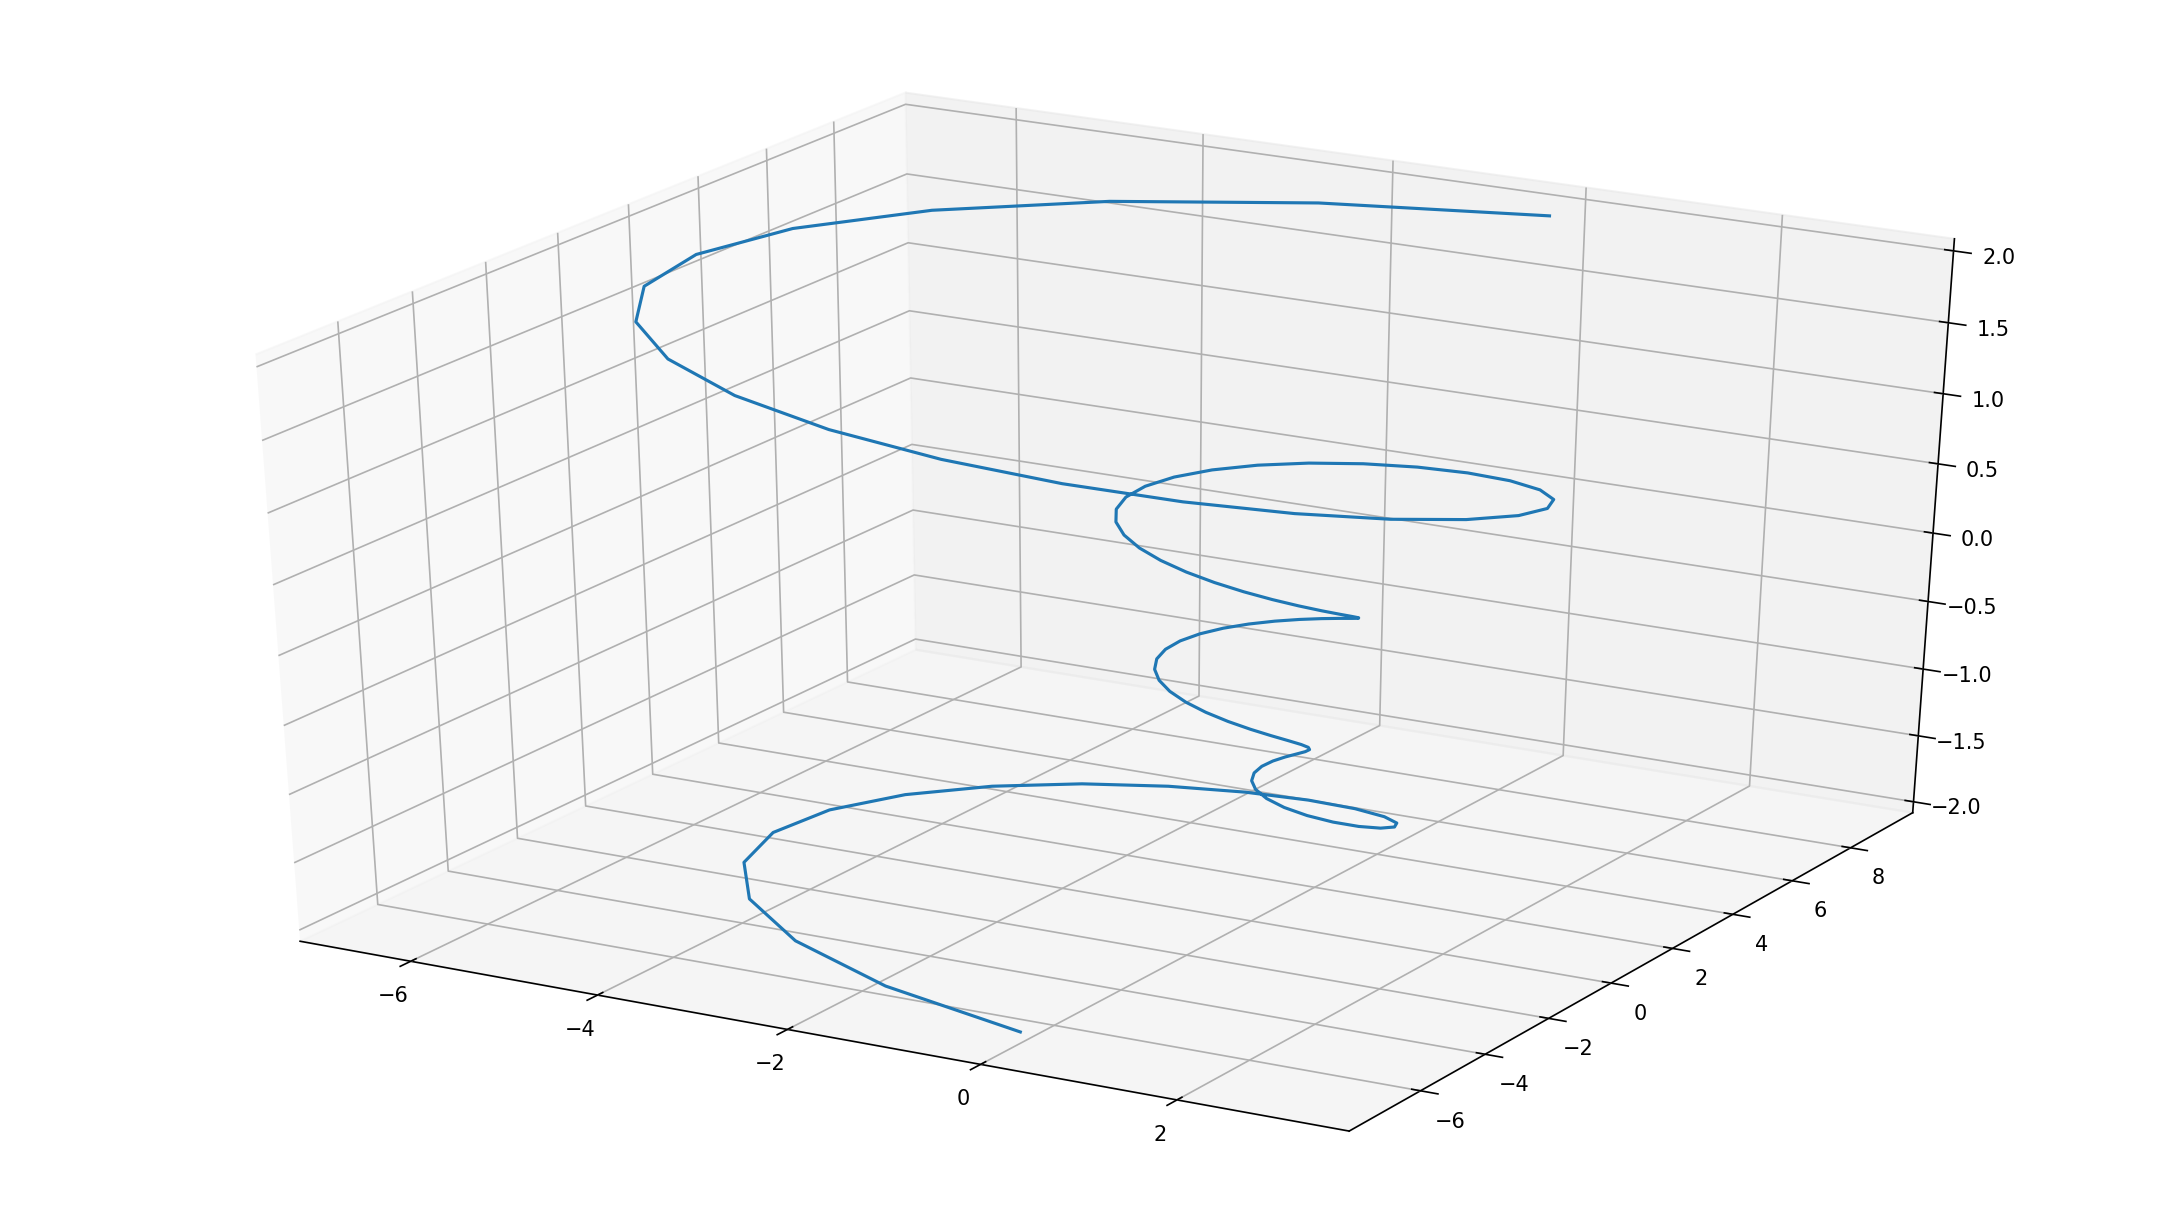
\includegraphics[width=\textwidth]{img/curve-1.png}
\caption{Térbeli ív szemléltetése.}
\label{fig:curve-1}
\end{figure}

A pontok által leírt ívet jeleníti meg egyetlen
töröttvonalként, de a \texttt{matplotlib} segítségével akár elhelyezhetjük rajta az adott diszkrét
pontokat is (\ref{fig:curve-2}. ábra):
\begin{python}
fig = plt.figure(figsize=(18.5, 10.5), dpi=150)
ax = fig.add_subplot(111, projection='3d')

theta = np.linspace(-4 * np.pi, 4 * np.pi, 100)
zline = np.linspace(-2, 2, 100)
r = z**3 + 1
xline = r * np.sin(theta)
yline = r * np.cos(theta)
ax.plot(xline, yline, zline)

zpoints = np.linspace(-2, 2, 100)
xpoints = r * np.sin(theta)
ypoints = r * np.cos(theta)
ax.scatter3D(xpoints, ypoints, zpoints, c=z, cmap="Reds")
plt.show()
\end{python}

\begin{figure}[h!]
\centering
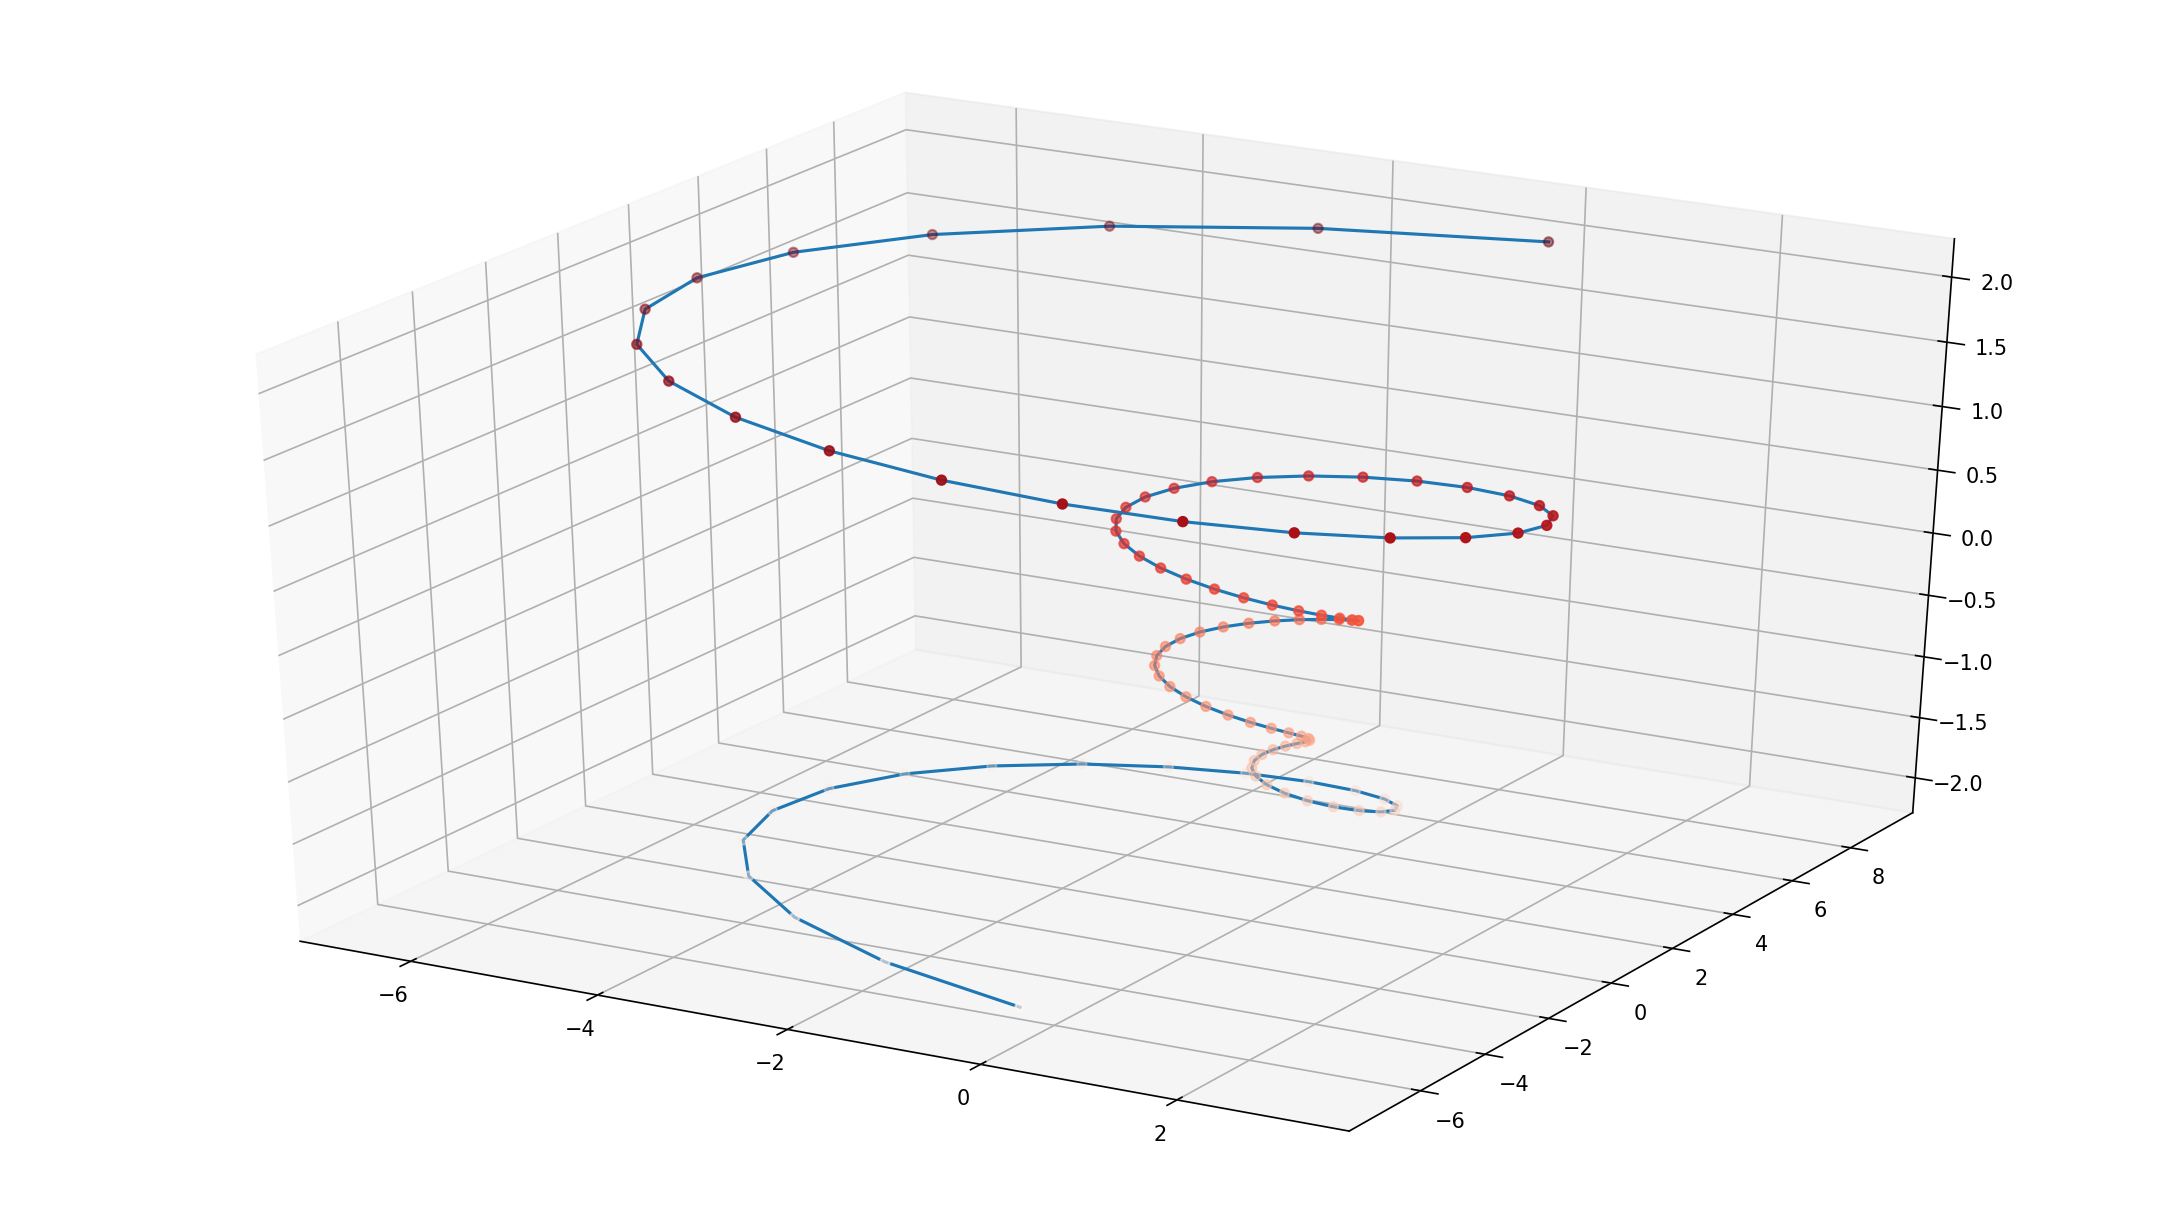
\includegraphics[width=\textwidth]{img/curve-2.png}
\caption{Térbeli ív szemléltetése diszkrét pontokkal együtt.}
\label{fig:curve-2}
\end{figure}
    
Megtehetjük azt is hogy cak a pontokat helyezzük el a 3D-s térben (\ref{fig:curve-3}. ábra):
\begin{python}
fig = plt.figure(figsize=(18.5, 10.5), dpi=150)
ax = fig.add_subplot(111, projection='3d')

theta = np.linspace(-4 * np.pi, 4 * np.pi, 100)
r = z**3 + 1
zpoints = np.linspace(-2, 2, 100)
xpoints = r * np.sin(theta)
ypoints = r * np.cos(theta)
ax.scatter3D(xpoints, ypoints, zpoints, c=z, cmap="hsv")
plt.show()
\end{python}

\begin{figure}[h!]
\centering
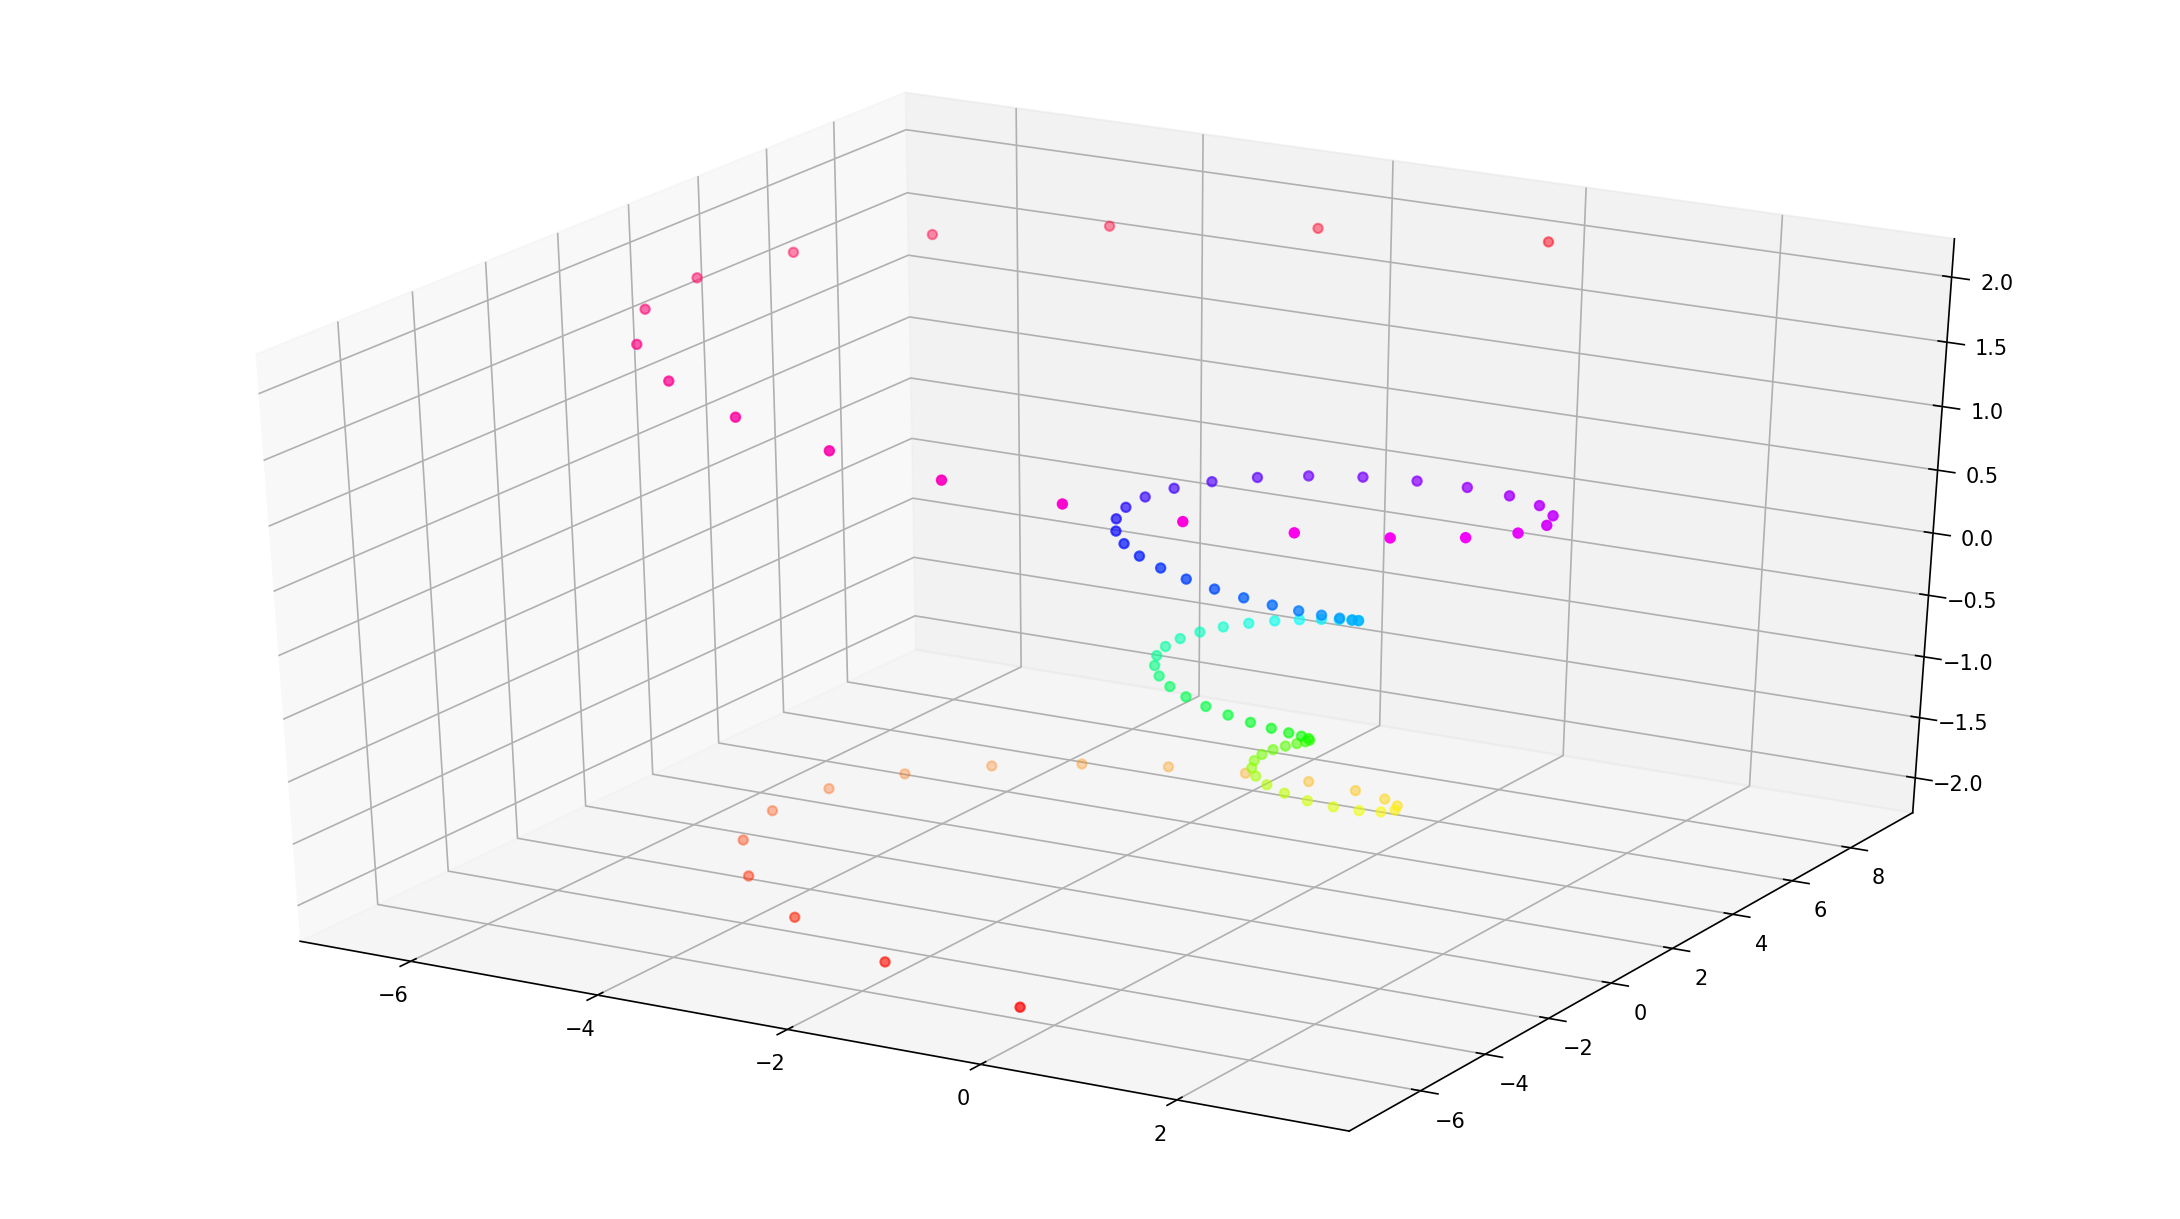
\includegraphics[width=\textwidth]{img/curve-3.png}
\caption{Térbeli pontok szemléltetése HSV színezéssel.}
\label{fig:curve-3}
\end{figure}
    
    Egy felületet megjeleníthetünk többféleképpen is a \textbf{wireframe}
segítségével egy háló szerűen, míg a \textbf{surface} használatával
egybefüggő felületként. A következő példában már a kapott térbeli felületi elforgatása is szerepel:
\begin{python}
def f(x, y):
    return np.sin(np.sqrt(x ** 2 + y ** 2))

x = np.linspace(-6, 6, 30)
y = np.linspace(-6, 6, 30)

X, Y = np.meshgrid(x, y)
Z = f(X, Y)

plt.figure(figsize=(18.5, 10.5), dpi=150)
ax = plt.axes(projection='3d')
ax.plot_surface(X, Y, Z, rstride=1, cstride=1,
                cmap='viridis', edgecolor='none')
ax.set_title('surface');
ax.view_init(60, 35)
\end{python}
Az így megjelenített felület \aref{fig:curve-4}. ábrán látható.

\begin{figure}[h!]
\centering
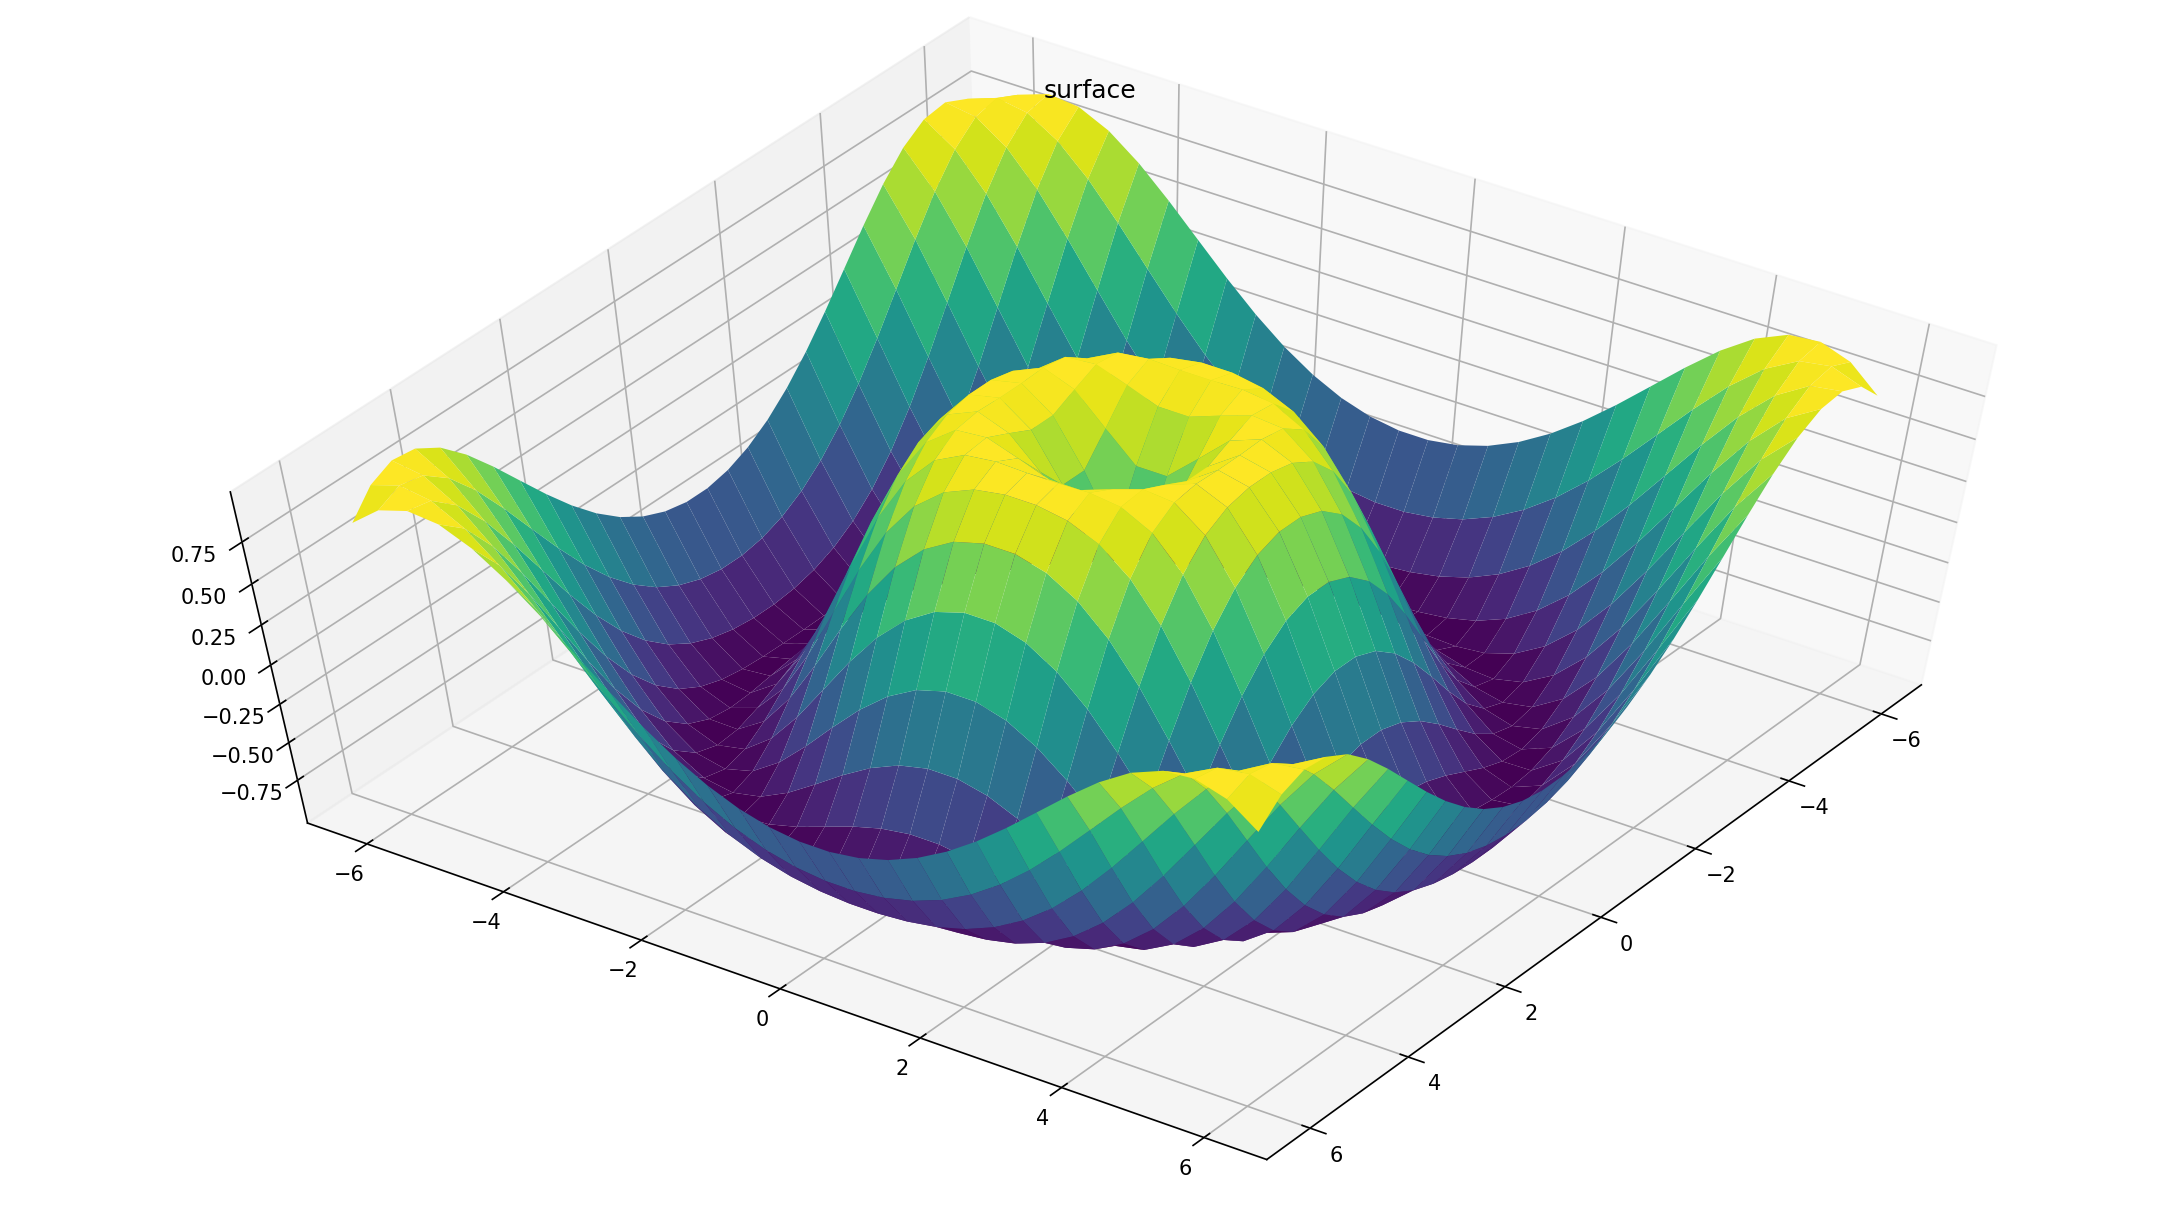
\includegraphics[width=\textwidth]{img/curve-4.png}
\caption{Térbeli felület megjelenítése.}
\label{fig:curve-4}
\end{figure}
    
    Sok más további lehetőséget is kínál a matplotlib, például megjeleníthetünk
3d-ben 2-ds adatokat, vagy készíthetünk 3d-s hisztogrammot több adattal,
de a fent említettek talán a legfontosabbak és legtöbbet használtak.

\Section{Interaktív widgetek Jupyter-ben}

Az interaktív plotokról csak említés szintjén esik szó a dolgozatban, hiszen ezek
készítését nem a Python, hanem a Jupyter notebook és a IPython kernel
teszi lehetővé. Az
\texttt{interact} segítségével tudunk interaktív dolgokat készíteni, például azért, hogy több adatra megnézhessük egy függvény képét. A következő
példában különböző hatvány függvényeket lehet megnézni, és a csúszka
segítségével lehet beállítani a hatvány kitevőt:
\begin{python}
from __future__ import print_function
from ipywidgets import interact, interactive, fixed, interact_manual
import ipywidgets as widgets
import matplotlib.pyplot as plt
import numpy as np
from ipywidgets import Button, Layout

def f(y):
    x = np.linspace(-100, 100, 100)
    plt.figure(figsize=(14, 7), dpi=150)
    plot = plt.plot(x, x**y)
    plt.show()

interact(f, y=widgets.IntSlider(min=1, max=30, step=1, value=0));
\end{python}
    
A minta számot is beállíthatjuk egy ilyen csúszkával és ezzel a pontosságot tudjuk szabályozni:
\begin{python}
def f(y):
    x = np.linspace(-10, 10, y)
    plt.figure(figsize=(14, 7), dpi=150)
    plot = plt.plot(x, x**2, 'o', color="green")
    plt.show()

interact(f, y=widgets.IntSlider(min=1, max=200, step=1, value=0));
\end{python}
Egy értékbeállítást láthatunk \aref{fig:interact-1}. ábrán.

\begin{figure}[h!]
\centering
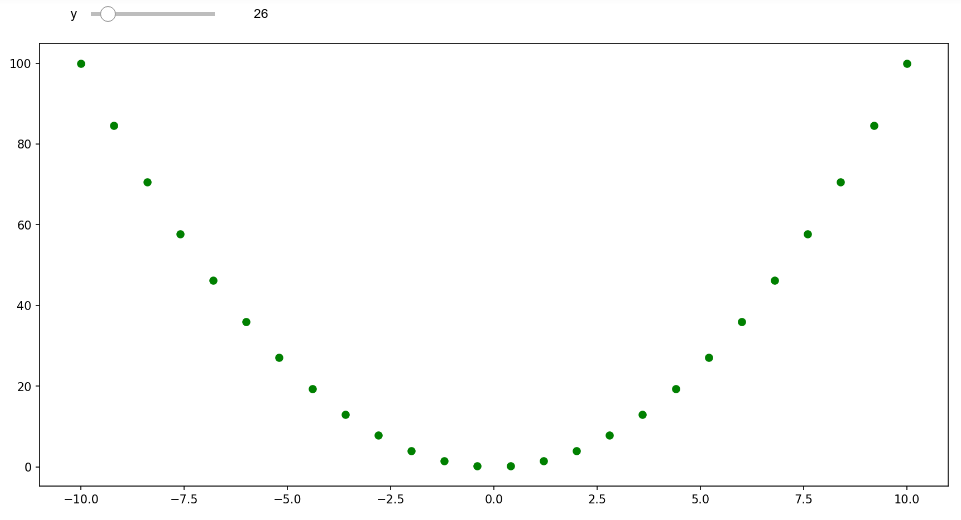
\includegraphics[width=\textwidth]{img/interact-1.png}
\caption{Csúszka használata.}
\label{fig:interact-1}
\end{figure}

    Az interaktivitásnak sok további formája van. Például
vannak még igaz/hamis értékekre állítható jelölőnégyzet  (\texttt{Checkbox}), szöveges
bevitelre alkalmas mező (\texttt{Text}), lenyíló
lista (\texttt{Dropdown}). Itt szerepel egy kis
példa egy szöveges mezőre mely összead két számot.
\begin{python}
def f(a, b):
    if a == "":
        x = 0
    else:
        x = float(a)
    if b == "":
        y = 0
    else:
        y = float(b)
    print(x + y)

interact(f, a="", b="");
\end{python}
    Fontos megjegyezni, hogy a beírt dolgok szövegként kerülnek átadásra, ezért szükség lehet azok számmá való konvertálására, ahogy az előbbi példában is látható.
    
    Megvalósításából fakadóan ezek az interaktív eszközök használhatóak 3D plotoknál, illetve más helyeken is.
Különösen hasznos lehet például térben ábrázolt felület forgatásánál. Ez az alábbi kódrészlettel valósítható meg.
\begin{python}
from mpl_toolkits.mplot3d import axes3d

def f(x, y):
    return np.sin(np.sqrt(x ** 2 + y ** 2))

def g(angle1, angle2):
    x = np.linspace(-6, 6, 30)
    y = np.linspace(-6, 6, 30)

    X, Y = np.meshgrid(x, y)
    Z = f(X, Y)

    plt.figure(figsize=(14, 7), dpi=150)
    ax = plt.axes(projection='3d')
    ax.plot_surface(X, Y, Z, rstride=1, cstride=1,
                    cmap='viridis', edgecolor='none')
    ax.set_title('surface');
    ax.view_init(angle1, angle2)
    
interact(g,
    angle1=widgets.IntSlider(min=0, max=360, step=1, value=0,
        layout=Layout(width="600px")),
    angle2=widgets.IntSlider(min=0, max=360, step=1, value=0,
        layout=Layout(width="600px")));
\end{python}
